\section{Auswertung}

Zunächst wird im Versuch die Winkelrichtgröße $D$ und das
das Eigenträgheitsmoment der Drillachse $I_D$ bestimmt. %komma statt Punkt, Aufzählung
Anschließend das Trägheitsmoment einer Kugel und eines Zylinders (\emph{grau}).
Dazu kommt noch das Trägheitsmomente von einer Holzpuppe in zwei verschieden Positionen. %Ausdruck
Da das Trägheitsmoment nicht direkt gemessen werden kann, wurden immer
die Schwingungsdauer $T$ von $5$ Schwingungen gemessen.
Um so dann auf das Trägheitsmoment zu schließen.  %kompliziert formuliert

\subsection{Bestimmung der Winkelrichtröße $D$}

Die Winkelrichtgröße $D$ kann auf zwei verschiedene Wege bestimmt werden.
Zum einem durch eine passive und zum andern durch eine dynamische Methode. %wieso passiv?
Beide Methoden werden im Anschluss genauer erklärt werden.

\subsubsection{Passive Methode}

Die Passive oder auch als statisch bezeichnete Methode wird mittels einem Drehmoment (gemessen mit einer Federwaage)
das für eine Auslenkung der Torsionsfeder sorgt gemessen. %Ausdruck
Wichtig dabei ist, dass die Federwaage immer orthogonal zum Radius steht.
Denn das Drehmoment errechnet sich mit $\vec{M}=\vec{r}\times\vec{F}$, durch
eine orthogonale Stellung von $\vec{r}$ und $\vec{F}$ kann mit den Beträgen %das hab ich in der Durchführung schon beschrieben
gerechnet werden und ergibt den Zusammenhang $M=rF$.
Im Versuch wurden folgende Werte bestimmt:


\begin{table}
\centering
\caption{Messung der Kraft für eine Auslenkung}
\label{tab: winkelricht}
\renewcommand{\arraystretch}{1.2}
\begin{tabular}{lcr}
	\toprule
	Abstand in $\si{\meter}$ & Winkel in $\mathrm{rad}$ & Kraft in $\si{\newton}$ \\
	\midrule
	$\num{1.01e-1}$ & $\frac{\pi}{6}$ & $\num{1.40e-1}$ \\
	$\num{1.01e-1}$ & $\frac{\pi}{3}$ & $\num{2.40e-1}$ \\
	$\num{1.01e-1}$ & $\frac{\pi}{2}$ & $\num{3.20e-1}$ \\
	$\num{1.01e-1}$ & $\frac{2\pi}{3}$ & $\num{4.60e-1}$ \\
	$\num{1.58e-1}$ & $\frac{\pi}{6}$ & $\num{6e-2}$ \\
	$\num{1.58e-1}$ & $\frac{\pi}{3}$ & $\num{1.2e-1}$ \\
	$\num{1.58e-1}$ & $\frac{\pi}{2}$ & $\num{2.20e-1}$ \\
	$\num{1.58e-1}$ & $\frac{2\pi}{3}$ & $\num{3e-1}$ \\
	$\num{2.41e-1}$ & $\frac{\pi}{6}$ & $\num{2.00e-2}$ \\
	$\num{2.41e-1}$ & $\frac{\pi}{3}$ & $\num{8.00e-2}$ \\
	$\num{2.41e-1}$ & $\frac{\pi}{2}$ & $\num{1.2e-1}$ \\
	$\num{2.41e-1}$ & $\frac{2\pi}{3}$ & $\num{2.00e-2}$ \\
	\bottomrule
\end{tabular}
\end{table}

Mit dem Zusammenhang

\begin{equation*}
D=\frac{M}{\phi}=\frac{Fr}{\phi}
\end{equation*}

ergibt sich dann, für jede Einzelne der insgesamt $n$ Messungen ein Wert für die Winkelrichtgröße.
Diese wurden anschließend durch,

\begin{equation}
\label{eq:mittel}
\bar{x}=\frac{1}{n}\sum_{i=1}x_i
\end{equation}

gemittelt, mit der dazugehörigen Abweichung

\begin{equation}
\label{eq:stand_ab}
\bar{\sigma}_{\bar{x}}=\sqrt{\frac{1}{n(n-1)}\sum_{i=1}^{n}(x_i-\bar{x})^2}.
\end{equation}

Es ergibt sich dann für die Winkelrichtgröße der Wert:

\begin{equation}
\label{eq:winkel_passiv}
D_{passiv}=\left(\num{2.03e-2} \pm \num{1.22e-3}\right)\si{\newton\meter} %Fehler und Bestwert unbedingt in gleicher Präzision
\end{equation}

\subsubsection{Dynamische Methode}

Bei der dynamischen Methode wird die Schwingungsdauer von %können zwei kleine Zylinder eine Schwingungsdauer haben?
zwei kleinen Zylindern ($m_1$ und $m_2$), die symmetrisch zum Mittelpunktes
eines Stabes befestigt werden, gemessen. Durch Verschiebung der Massen,
ergibt sich eine Vielzahl von Messwerten, die im Anhang eingesehn %"Vielzahl" unpassend
werden können.
Diese wurden anschließend gemittelt mit \eqref{eq:mittel} und \eqref{eq:stand_ab}.
Das Resultat ist in der Tabelle dargestellt: %referiere hier auf die Tabelle

\begin{table}
\centering
\caption{Gemittelte Schwingungsdauer für die dynamische Methode}
\label{tab: winkel_dynamisc}
%\renewcommand{\arraystretch}{1.2}
\begin{tabular}{lr}
	\toprule
	$\bar{T}$ in $\si{\per\second}$ &  $\sigma_{\bar{T}}$ in $\si{\per\second}$ \\
	\midrule
	\num{2.52} & \num{6.43e-3} \\
	\num{3.23} & \num{9.16e-3} \\
	\num{3.65} & \num{5.89e-3} \\
	\num{4.08} & \num{3.57e-3} \\
	\num{4.56} & \num{6.82e-3} \\
	\num{5.09} & \num{2.83e-2} \\
	\num{5.56} & \num{3.33e-2} \\
	\num{6.05} & \num{1.07e-2} \\
	\num{6.59} & \num{8.64e-3} \\
	\num{7.07} & \num{3.31e-3} \\
	\bottomrule
\end{tabular}
\end{table}

Mit den Schwingungsdauern und dem Gesetz

\begin{equation*}
T=2\pi\sqrt{\frac{I}{D}} \quad \Leftrightarrow \quad I=\frac{T^2 D}{4\pi^2}
\end{equation*}

kann auf die Winkelrichtgröße geschlossen werden.
Da die Zylinder von der Drehachse verschoben sind, macht man sich den
Satz von Steiner \eqref{eq: steiner} zu nutze und erhält den Zusammenhang: %kompliziert formuliert

\begin{equation}
\label{eq:gerade}
\frac{T^2D}{4\pi^2}=I_s+ma^2\quad \Leftrightarrow \quad T^2=\frac{I_s 4\pi^2}{D}+\frac{4m_g\pi^2}{D}a^2
\end{equation}

Dabei sei $m_g=m_1+m_2=\num{222.51e-2}\si{\meter}+\num{223.46e-2}\si{\meter}$.
Offensichtlich ergibt sich eine Gleichung für eine Gerade, die mittels linearer
Regression angenährt werden kann. %besser: zwischen T^2 und a^2 besteht einer linearer Zusammenhang, die Funktionsparameter lassen sich mittels linearer Regerssion bestimmen...
Dazu verwendet man aus der Regressionsrechnung
die Annäherung um die Steigung $m$

\begin{equation*}
m=\frac{\bar{xy}-\bar{x}\bar{y}}{\bar{x^2}-\bar{x}^2}
\end{equation*}

zu bestimmen, mit dem dazugehörigen Fehler

\begin{equation*}
\sigma_m=\sqrt{\frac{\sigma^2}{N(\bar{x^2}-\bar{x}^2)}}.
\end{equation*}

Nach Ausführung der Regressionsrechnung ergibt sich als Wert
\begin{equation}
\label{eq: steigung}
m=\left(\num{741.2}\pm\num{3.4}\right) \si{\kilogram\per\newton\meter}.
\end{equation}

Da es sich bei \eqref{eq:gerade} um eine Gerade handelt muss gelten:

\begin{equation*}
m=\frac{4m_g\pi^2}{D}
\end{equation*}

Damit wird die Winkelrichtgröße dynamisch bestimmt, denn es gilt %dynamisch bestimmt?

\begin{equation*}
D=\frac{4m_g\pi^2}{m}.
\end{equation*}

Er ergibt sich:

\begin{equation}
\label{winkelrichtgroesse_dynamisch}
D_{dynam}=\left(\num{2.38e-2} \pm \num{1.10e-4}\right)\si{\newton\meter}
\end{equation}

Da die Abweichung von $D_{dynam}$ kleiner ist als von $D_{passiv}$ wird
diese in folgenden Rechnungen genutzt.
Dabei sei ab sofort $D=D_{dynam}$.


\subsection{Bestimmung des Eigenträgheitsmoment $I_D$}

Auch bei der Bestimmung des Eigenträgheitsmomentes machen wir uns die
Geradengleichung \eqref{eq:gerade} und dessen lineare Regression zunutze.
Denn durch Betrachtung des $y$-Achsenabschnitt der Geraden kann auf das Eigenträgheitsmoment der Drillachse geschlossen werden. %kompliziert
Dazu

\begin{equation*}
b=\frac{4\pi^2}{D}\left(I_D+I_Z\right) \quad \Leftrightarrow \quad I_D=\frac{D}{4\pi^2}b-I_Z
\end{equation*}

Dabei sei $I_Z$ das Trägheitsmoment der kleinen Zylinder.%Soll ich die noch dahin schreiben ?

Aus der Regressionsrechnung ergibt sich der Zusammenhang

\begin{equation*}
b=\frac{\bar{x^2}\bar{y}-\bar{x}\bar{xy}}{\bar{x^2}-\bar{x}^2}
\end{equation*}

für den $y$-Achsenabschnitt und der dazugehörigen Abweichung

\begin{equation*}
\sigma_b=\sqrt{\frac{\sigma^2}{N\left(\bar{x^2}-\bar{x}^2\right)}}.
\end{equation*}

Rechnerisch ergibt sich:

\begin{equation}
\label{eq:y_achsenabschnitt}
b=\left(\num{4.64}\pm\num{0.12}\right) \si{\meter}
\end{equation}

Mit dem theoretisch errechneten Wert für das Trägheitsmoment der kleinen Zylinder
(mittels \eqref{eq:traeg_zylinder_schwer}) ergibt sich für das
Eigenträgheitsmoment der Drillachse:

\begin{equation}
\label{eq:eigentraegheitsmoment}
I_D=\left(\num{0.003}\pm\num{0.000}\right) \si{\kilogram\meter\squared}
\end{equation}


Abschließend wird der schon benutzte lineare Zusammenhang zwischen $T^2$ und $a^2$ grafisch aufgezeigt.

\begin{figure}
  \centering
  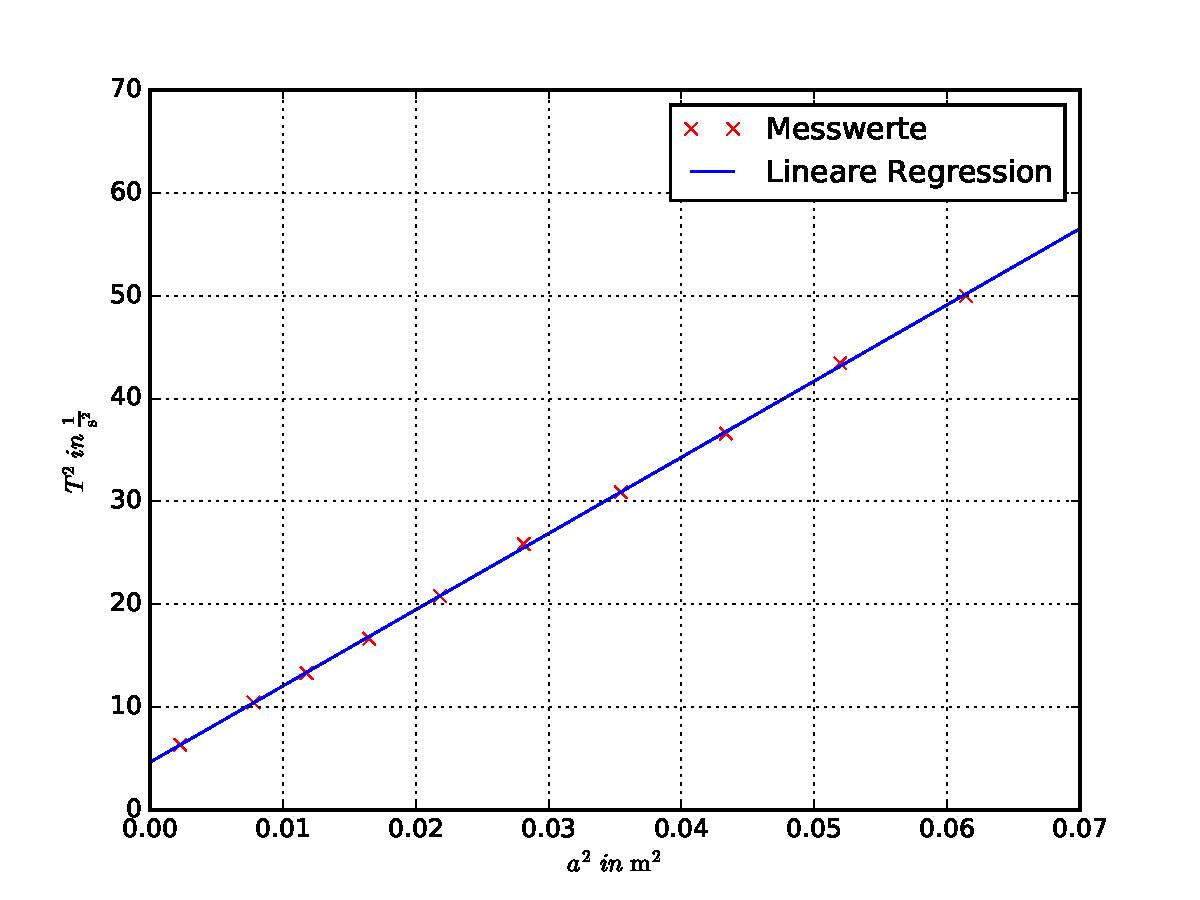
\includegraphics[width=0.9\textwidth]{pics/lineare_regression.pdf}
  \caption{Zusammenhang zwischen $T^2$ und $a^2$}
  \label{fig:zusammenhang_a_T}
\end{figure}


\subsection{Experimentelle Bestimmung des Trägheitsmomentes von Zylinder und Kugel}

Um das Trägheitsmoment zu bestimmen, wird der Zusammenhang

\begin{equation*}
I_{körper}=\frac{T^2 D}{4\pi^2}-I_D
\end{equation*}
genutzt.
Am Ende jedes Unterkapitels soll ein Vergleich zwischen den
Trägheitsmomenten die aus der Theorie folgen und den
experimentellen Trägheitsmomenten folgen. %Ausdruck

\subsubsection{Trägheitsmoment des Zylinder}

Die gemessenen Schwingungsdaueren sind im Anhang nachzulesen.
Als gemittelter Wert ergibt sich:

\begin{equation*}
\bar{T}_{zylin}=\left(\num{1.17}\pm\num{0.00}\right) \si{\per\second}
\end{equation*}

Damit folgte für das Trägheitsmoment:

\begin{equation}
\label{eq:traeg_zylinder_grau_exp}
I_{zylin}=\left(\num{0.0008}\pm\num{0.0000}\right) \si{\kilogram\meter\squared}
\end{equation}

Für die theoretische Berechnung werden die Maße und Masse des Zylinders benötigt.
Gemessen wurde:

\begin{align*}
\text{Maße} \quad &\\
d&=\num{3.49e-2}\si{\meter}\\
h&=\num{3.01e-2}\si{\meter}\\
\text{Masse} \quad &\\
m_{zyl}&=\num{1005.8}\si{\gram}
\end{align*}

Da es sich hier um eine Drehung um die Symmetrieachse handelt, wird zu
theoretischen Berechnung \eqref{eq:traeg_zylinde} genutzt.
Das resultierende Ergebnis lautet:

\begin{equation}
\label{eq:traeg_zylinder_theo}
I_{zylin \,theo}= \num{0.0006}\si{\kilogram\meter\squared}
\end{equation}

Die Abweichung vom experimentellen Resultat zur Theorie beläuft sich auf $\approx +33 \%$ %Ich würde den qualitativen Vergleich zwischen Theorie und Experiment in der Diskussion anstellen

\subsubsection{Trägheitsmoment der Kugel}

Bei der Bestimmung des Trägheitsmomentes einer Kugel wird genauso vorgegangen, wie bei
der Bestimmung für den Zylinder. %Ausdruck
 Auch hier sind die gemessenen Schwingungsdaueren im Anhang einzusehen.
Als gemittelter Wert ergibt sich:

\begin{equation*}
\bar{T}_{kugel}=\left(\num{1.66}\pm\num{0.00}\right) \si{\per\second}
\end{equation*}

Daraus folgt für das Trägheitsmoment:

\begin{equation}
\label{eq:traeg_kugel_exp}
I_{kugel}=\left(\num{0.002}\pm\num{0.000}\right) \si{\kilogram\meter\squared}
\end{equation}

Um das theoretische Trägheitsmoment zu bestimmen, werden die Abmessungen und das Gewicht der Kugel benötigt:

\begin{align*}
\text{Abmessung} \quad &\\
d&=\num{13.78e-2}\si{\meter}\\
\text{Gewicht} \quad &\\
m_{zyl}&=\num{812.40}\si{\gram}
\end{align*}

Als theoretische Grundformel wird \eqref{eq:traeg_kugel} genutzt.
Es resultiert

\begin{equation}
\label{eq:traeg_kugel_theo}
I_{kugel \,theo}= \num{0.002}\si{\kilogram\meter\squared}
\end{equation}

als theoretisches Trägheitsmoment.

Abschließend gilt es noch zu erwähnen, dass es keinen Unterschied
zwischen theoretischen und experimentellen Trägheitsmoment gibt. %was heißt das?

\subsection{Trägheitsmoment der Modellpuppe}

Wie auch bei dem vorherigen Körpern wird zu Bestimmung des Trägheitsmomentes
die Schwingungsdauer der Puppe gemessen. %falschrum

Der wesentliche Unterschied zu den vorhrigen Körpern ist, der Vergleich mit den
theoretischen Werten. %ausdruck
Denn bei der Berechnung muss die Form der Puppe
durch bekannte Körper (Zylinder und Kugeln) angenährt werden.
Da die einzelnen Körperteile nicht an jeder Stelle die gleichen Maße haben,
werden meheree Werte gemessen (siehe Anhang) und dann gemittelt.
Es ergeben sich folgende Abmessungen für die Körperteile:

\begin{align*}
\text{Abmessung} \quad &\\
r_{kopf}&=\left(\num{0.027}\pm\num{0.002}\right)\si{\meter}\\
r_{arm}&=\left(\num{0.015}\pm\num{0.001}\right)\si{\meter}\\
r_{torso}&=\left(\num{0.035}\pm\num{0.004}\right)\si{\meter}\\
r_{bein}&=\left(\num{0.018}\pm\num{0.001}\right)\si{\meter}\\
\text{Gewicht} \quad &\\
m_{puppe}&=\num{161.90}\si{\gram}
\end{align*}

Für spätere Berechnung wird die Puppe, wie auf der folgenden Abbildung zusehen geometrisch angenährt: %ref


\begin{figure}
  \centering
  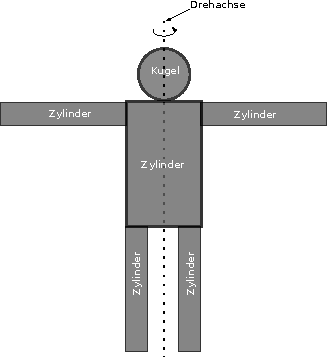
\includegraphics[width=0.6\textwidth]{pics/puppe.pdf}
  \caption{Annäherung der Puppe}
  \label{fig:approx_puppe}
\end{figure}

\subsubsection{Position 1}

Die Haltung der Puppe in Position 1 ist in Abbildung \ref{fig:pup1} dargestellt.
Die gemessenen Schwingungsdauern sind im Anhang aufgelistet.
Als Mittelwert ergibt sich:

\begin{equation*}
\bar{T}_{puppe\, p1}=\left(\num{0.64}\pm\num{0.00}\right) \si{\per\second}
\end{equation*}

Daraus resultiert für das Trägheitsmoment:

\begin{equation}
\label{eq:traeg_puppe_p1}
I_{puppe \,p1}= \left(\num{0.0002}\pm\num{0.0000}\right)\si{\kilogram\meter\squared}
\end{equation}

Bei der Berechnung des theoretischen Trägheitsmomentes, macht man sich
das additive Verhalten der Trägheitsmomente zu nutzen.
Dabei ist jedoch zu beachten, dass bei den Armen und Beinen der
Satz von Steiner zu berücksichtigen ist. %Ausdruck
 Dabei sind die Verschiebungen zur Drehachse
\begin{align*}
a_{arm}&=\num{9.27e-2}\si{\meter}\\
a_{bein}&=\num{1.19e-2}\si{\meter}
\end{align*}

Des Weiteren wird für den Satz von Steiner die Masse von Armen und Beinen benötigt.
Diese werden bestimmt, indem man das Teilvolumen von Arm und Bein zum Gesamtvolumen bestimmt. %Ausdruck
Das Teilvolumen wird dann anschließend mit der Masse der Puppe multipliziert.

Für einen Arm ergibt sich
\begin{align}
\begin{aligned}
\label{eq:masse_arm}
\text{prozentualer} Anteil \quad &\left(10\pm\num{1}\right)\% \\
\text{Masse Arm} \quad &\left(\num{0.016}\pm\num{0.002}\right)\si{\kilogram}
\end{aligned}
\end{align}

und für ein Bein

\begin{align}
\begin{aligned}
\label{eq:masse_bein}
\text{prozentualer} Anteil \quad &\left(16\pm\num{2}\right)\% \\
\text{Masse Bein} \quad &\left(\num{0.026}\pm\num{0.003}\right)\si{\kilogram}.
\end{aligned}
\end{align}

Nach der Theorie hat die Puppe in Position $1$ ein Trägheitsmoment von

\begin{equation*}
\bar{T}_{puppe\, p1\,theo}=\left(\num{1.55e-5}\pm\num{0.27e-5}\right) \si{\kilogram\meter\squared}.
\end{equation*}

Der Unterschied zwischen Theorie und Praxis liegt bei $\approx +1200 \%$. %s.o.

\subsubsection{Position 2}
Die Haltung der Puppe in Position 2 ist in Abbildung \ref{fig:pup2} zusehen.
Die gemessenen Schwingungen sind im Anhang abgedruckt. %musst nicht immer auf den Anhang verweisen denke ich
Als gemittelte Schwingungsdauer errechnet sich:

\begin{equation*}
\bar{T}_{puppe\, p2}=\left(\num{0.91}\pm\num{0.00}\right) \si{\per\second}
\end{equation*}

Damit folgt für das Trägheitsmoment

\begin{equation}
\label{eq:traeg_puppe_p2}
I_{puppe \,p2}= \left(\num{0.0005}\pm\num{0.0000}\right)\si{\kilogram\meter\squared}
\end{equation}

Da bei dieser Position nur die Beine ihre Position geändert haben, ändert
sich ihr Abstand zu der Drehachse auf $a_{beine}=\num{6.77e-2}\si{\meter}$.
Sonst bleiben Massen und Abstände gleich.

Für das theoretische Trägheitsmoment folgt

\begin{equation*}
\bar{T}_{puppe\, p2\,theo}=\left(\num{0.0002}\pm\num{0.0000}\right) \si{\kilogram\meter\squared}.
\end{equation*}

Die Abweichung von dem experimentellen und theoretischen Ergebnis ist
somit $\approx +250 \%$. %s.o.
